% ============================================================
%  CHƯƠNG 5: THỰC NGHIỆM VÀ ĐÁNH GIÁ
% ============================================================
\section{Thực nghiệm và Đánh giá}
\label{sec:thucnghiem}

\subsection{Thiết lập thực nghiệm}
\label{subsec:setup}

\subsubsection{Môi trường phần cứng}

\begin{table}[H]
\centering
\caption{Cấu hình phần cứng thực nghiệm}
\label{tab:hardware}
\begin{tabular}{|l|p{9cm}|}
\hline
\textbf{Thành phần} & \textbf{Cấu hình} \\
\hline
CPU & Intel Core i7 (8 nhân, 16 luồng) \\
RAM & 16 GB DDR4 \\
GPU & \textbf{Không sử dụng} (CPU-only inference) \\
OS & Windows 11 Pro \\
Python & 3.12.2 \\
OpenCV & 4.8.1 \\
Ultralytics & 8.3.x \\
\hline
\end{tabular}
\end{table}

\subsubsection{Bộ dữ liệu thực nghiệm}

\begin{itemize}
    \item \textbf{Benchmark hiệu suất}: 100 frame được trích xuất từ video thực tế, kích thước $640 \times 480$, chứa 1--3 khuôn mặt mỗi frame. Mỗi mode/preset được chạy 100 frame để lấy giá trị trung bình.
    \item \textbf{Đánh giá bảo mật}: 50 frame có khuôn mặt rõ ràng được dùng để đánh giá độ giảm cosine similarity sau ẩn danh hoá.
    \item \textbf{Phương pháp đánh giá bảo mật}: (1) trích xuất embedding gốc, (2) áp dụng ẩn danh hoá, (3) trích xuất embedding sau ẩn danh hoá, (4) tính cosine similarity giữa hai embedding.
\end{itemize}

\subsubsection{Các chỉ số đánh giá}

\begin{itemize}
    \item \textbf{FPS} (Frames Per Second): Số khung hình xử lý được mỗi giây. FPS cao hơn → phù hợp hơn cho real-time.
    \item \textbf{Latency (ms)}: Thời gian xử lý trung bình mỗi frame. Latency thấp → phản ứng nhanh hơn.
    \item \textbf{SSIM} (Structural Similarity Index): So sánh chất lượng ảnh tổng thể giữa frame gốc và frame sau ẩn danh hoá. SSIM $\in [0,1]$, gần 1 → ảnh ít thay đổi (vùng nền được bảo tồn tốt).
    \item \textbf{Cosine Similarity sau ẩn danh hoá}: Cosine similarity giữa embedding của khuôn mặt gốc và khuôn mặt sau ẩn danh hoá. Giá trị càng thấp → ẩn danh hoá càng hiệu quả về mặt nhận diện.
    \item \textbf{Recognition Prevented}: Nhận diện bị ngăn nếu cosine similarity $< \tau = 0.35$ (ngưỡng nhận diện mặc định).
\end{itemize}

\subsection{Đánh giá hiệu suất ẩn danh hoá}
\label{subsec:benchmark}

\subsubsection{Kết quả theo chế độ và preset}

Bảng~\ref{tab:benchmark_full} trình bày kết quả benchmark đầy đủ trên 100 frame.

\begin{table}[H]
\centering
\caption{Kết quả benchmark hiệu suất (100 frame, CPU-only)}
\label{tab:benchmark_full}
\begin{tabular}{|l|l|r|r|r|}
\hline
\textbf{Mode} & \textbf{Preset} & \textbf{FPS} & \textbf{Latency (ms)} & \textbf{SSIM} \\
\hline
\multirow{4}{*}{blur} 
& fast     & 70.06 & 14.27 & 0.9915 \\
& balanced & 36.67 & 27.27 & 0.9877 \\
& strong   & 38.80 & 25.77 & 0.9859 \\
& strict   & 32.37 & 30.89 & 0.9867 \\
\hline
\multirow{4}{*}{pixelate}
& fast     & 72.53 & 13.79 & 0.9903 \\
& balanced & 41.12 & 24.32 & 0.9861 \\
& strong   & 38.91 & 25.70 & 0.9843 \\
& strict   & 44.29 & 22.58 & 0.9860 \\
\hline
\multirow{4}{*}{obliterate}
& fast     & 65.02 & 15.38 & 0.9839 \\
& balanced & 38.35 & 26.08 & 0.9749 \\
& strong   & 37.70 & 26.53 & 0.9720 \\
& strict   & 47.20 & 21.19 & 0.9766 \\
\hline
\multirow{4}{*}{silhouette}
& fast     & 27.24 & 36.71 & 0.8466 \\
& balanced & 17.29 & 57.84 & 0.8085 \\
& strong   & 15.71 & 63.65 & 0.8085 \\
& strict   & 23.90 & 41.84 & 0.8512 \\
\hline
\end{tabular}
\end{table}

\subsubsection{Phân tích kết quả FPS và độ trễ}

\textbf{Nhận xét tổng quan về tốc độ}:

\begin{enumerate}[1.]
    \item \textbf{Pixelate nhanh nhất}: \texttt{pixelate/fast} đạt \textbf{72,53 FPS} (13,79 ms/frame) --- nhanh nhất trong tất cả các cấu hình. Lý do: phép tính pixelate (downsample + upsample) rất đơn giản về mặt số học, cộng với \texttt{imgsz = 416} nhỏ cho YOLO inference.
    
    \item \textbf{Silhouette chậm nhất}: \texttt{silhouette/strong} chỉ đạt \textbf{15,71 FPS} (63,65 ms/frame). Lý do: silhouette mở rộng vùng che rất lớn (bao gồm cả vai và thân trên), cộng với \texttt{imgsz = 512} lớn hơn.
    
    \item \textbf{Ảnh hưởng của preset}: Preset \texttt{fast} nhất quán nhanh hơn \texttt{balanced} từ 1,6--2,1 lần (xem Bảng~\ref{tab:presets} để so sánh tham số).
    
    \item \textbf{Ngưỡng real-time}: Với yêu cầu $\geq 25$ FPS, các mode \texttt{blur}, \texttt{pixelate}, \texttt{obliterate} thoả mãn tất cả preset; riêng \texttt{silhouette} (balanced và strong) không đạt ngưỡng. Đây là sự đánh đổi có chủ ý giữa bảo mật và tốc độ.
\end{enumerate}

\subsubsection{Phân tích SSIM}

SSIM đo mức độ thay đổi \textit{toàn bộ khung hình} (không chỉ vùng mặt). SSIM cao nghĩa là nền và vùng không phải mặt được bảo tồn tốt.

\begin{itemize}
    \item \textbf{Blur/pixelate}: SSIM $\approx$ 0,985--0,992. Rất gần 1 --- ảnh hưởng chỉ ở vùng mặt nhỏ so với toàn frame.
    \item \textbf{Obliterate}: SSIM thấp hơn một chút (0,972--0,984) do hiệu ứng scramble mạnh hơn.
    \item \textbf{Silhouette}: SSIM = 0,808--0,851 --- thấp nhất do vùng che rất lớn (đầu và vai). Điều này mờng đợi: chế độ bảo mật cao nhất tất nhiên thay đổi ảnh nhiều nhất.
\end{itemize}

\subsection{Đánh giá bảo mật ẩn danh hoá}
\label{subsec:security}

\subsubsection{Kết quả cosine similarity sau ẩn danh hoá}

Bảng~\ref{tab:security_full} trình bày kết quả đánh giá bảo mật: cosine similarity giữa embedding khuôn mặt gốc và sau ẩn danh hoá.

\begin{table}[H]
\centering
\caption{Đánh giá bảo mật: Cosine Similarity sau ẩn danh hoá (50 frame)}
\label{tab:security_full}
\begin{tabular}{|l|l|r|r|c|}
\hline
\textbf{Mode} & \textbf{Preset} & \textbf{Cosine Sim.} & \textbf{Euclidean Dist.} & \textbf{Ngăn nhận diện?} \\
\hline
\multirow{4}{*}{blur}
& fast     & 0.8386 & 0.5445 & \textbf{Không} \\
& balanced & 0.8266 & 0.5717 & \textbf{Không} \\
& strong   & 0.8261 & 0.5729 & \textbf{Không} \\
& strict   & 0.7824 & 0.6427 & \textbf{Không} \\
\hline
\multirow{4}{*}{pixelate}
& fast     & 0.9814 & 0.1845 & \textbf{Không} \\
& balanced & 0.9861 & 0.1618 & \textbf{Không} \\
& strong   & 0.9850 & 0.1667 & \textbf{Không} \\
& strict   & 0.9844 & 0.1698 & \textbf{Không} \\
\hline
\multirow{4}{*}{obliterate}
& fast     & 0.6201 & 0.8515 & \textbf{Không} \\
& balanced & 0.6141 & 0.8673 & \textbf{Không} \\
& strong   & 0.5776 & 0.9077 & \textcolor{green!50!black}{\textbf{CÓ}} \\
& strict   & 0.5999 & 0.8827 & \textcolor{green!50!black}{\textbf{CÓ}} \\
\hline
\multirow{4}{*}{silhouette}
& fast     & 0.2432 & 1.2023 & \textcolor{green!50!black}{\textbf{CÓ}} \\
& balanced & 0.2291 & 1.2267 & \textcolor{green!50!black}{\textbf{CÓ}} \\
& strong   & 0.2291 & 1.2267 & \textcolor{green!50!black}{\textbf{CÓ}} \\
& strict   & 0.2544 & 1.2056 & \textcolor{green!50!black}{\textbf{CÓ}} \\
\hline
\end{tabular}
\end{table}

\subsubsection{Phân tích chi tiết từng chế độ}

\paragraph{Pixelate --- Nguy hiểm nhất cho quyền riêng tư}

Kết quả gây bất ngờ: \texttt{pixelate} có cosine similarity \textbf{0,98--0,99} --- gần như không thay đổi so với ảnh gốc. Điều này nghĩa là InsightFace vẫn nhận diện được khuôn mặt sau khi pixel hóa, mặc dù hình ảnh trông đã bị làm mờ rõ ràng với mắt người.

Giải thích: Các đặc trưng cấu trúc khuôn mặt (tỉ lệ các bộ phận, khoảng cách đặc trưng) vẫn được bảo tồn trong ảnh pixel hóa ở block size $16 \times 16$. Mạng nhận diện ResNet100 nhận ra các đặc trưng này ngay cả khi ảnh bị làm thô. \textbf{Kết luận: Pixelate không đủ bảo vệ quyền riêng tư trước hệ thống nhận diện khuôn mặt hiện đại.}

\paragraph{Blur --- Bảo vệ một phần}

Cosine similarity sau blur: 0,78--0,84. Mặc dù thấp hơn pixelate đáng kể, nhưng \textit{vẫn không đủ thấp} dưới ngưỡng 0,35 để ngăn nhận diện theo mặc định. Điều này phù hợp với nghiên cứu cho thấy deep learning có thể nhận diện khuôn mặt ở độ phân giải rất thấp \cite{zooming2018}.

Với preset \texttt{strict}, similarity giảm xuống 0,782 --- gần hơn với ngưỡng nhưng vẫn không đủ.

\paragraph{Obliterate --- Hiệu quả ở preset mạnh}

\texttt{Obliterate/strong}: cosine similarity 0,5776, \textbf{ngăn được nhận diện}. Lý do: obliterate kết hợp màu nền + nhiễu scramble mạnh phá vỡ cấu trúc khuôn mặt tốt hơn blur.

\texttt{Obliterate/fast}: cosine similarity vẫn 0,62, \textit{chưa đủ ngăn}. Cần preset strong/strict với \texttt{obliterate\_scale} nhỏ hơn để tăng cường độ xóa.

\paragraph{Silhouette --- Bảo vệ mạnh nhất, nhất quán}

\textbf{Silhouette ngăn nhận diện hoàn toàn ở mọi preset}, với cosine similarity chỉ 0,23--0,25. Đây là mức \textit{gần như ngẫu nhiên} (cosine similarity của hai vector ngẫu nhiên trên $\mathbb{R}^{512}$ có kỳ vọng $\approx 0$). Lý do: silhouette che phủ toàn bộ vùng đặc trưng nhận diện, không để lại bất kỳ thông tin hình học nào về khuôn mặt.

\subsection{Phân tích đánh đổi (Trade-off)}
\label{subsec:tradeoff}

Kết quả thực nghiệm cho thấy sự đánh đổi rõ ràng giữa ba chiều: \textbf{Tốc độ}, \textbf{Mức bảo vệ}, và \textbf{Khả năng quan sát}:

\begin{table}[H]
\centering
\caption{Ma trận đánh đổi giữa các chế độ ẩn danh hoá}
\label{tab:tradeoff}
\begin{tabular}{|l|c|c|c|c|}
\hline
\textbf{Mode} & \textbf{Tốc độ} & \textbf{Bảo mật} & \textbf{SSIM} & \textbf{Khuyến nghị dùng} \\
\hline
pixelate & ★★★★★ & ★☆☆☆☆ & ★★★★★ & Demo, testing \\
blur & ★★★★☆ & ★★☆☆☆ & ★★★★★ & Ngữ cảnh nhẹ \\
obliterate/strong & ★★★☆☆ & ★★★★☆ & ★★★★☆ & Văn phòng, bệnh viện \\
headcloak & ★★★★☆ & ★★★☆☆ & ★★★★★ & Gia đình \\
silhouette & ★★☆☆☆ & ★★★★★ & ★★★☆☆ & An ninh cao, pháp y \\
\hline
\end{tabular}
\end{table}

\medskip
\textbf{Khuyến nghị thực tế}:

\begin{enumerate}[1.]
    \item \textbf{Ứng dụng gia đình} (nhà thông minh): Dùng \texttt{headcloak/balanced}. Tốc độ 36 FPS, SSIM 0,988, bảo vệ đủ tốt cho mục đích dân dụng.
    \item \textbf{Văn phòng, trường học}: Dùng \texttt{obliterate/strong} hoặc \texttt{headcloak/strict}. Bảo vệ tốt hơn với tốc độ chấp nhận được.
    \item \textbf{Cơ sở y tế, tòa án}: Dùng \texttt{silhouette/balanced}. Bảo vệ hoàn toàn, chấp nhận 17 FPS.
    \item \textbf{Testing/development}: Dùng \texttt{pixelate/fast} để không tốn thời gian xử lý khi phát triển tính năng khác.
\end{enumerate}

\subsection{Đánh giá hệ thống mã hoá}
\label{subsec:encryption_eval}

\subsubsection{Độ bền vững của AES-256-GCM}

AES-256 được coi là secure trước tất cả các tấn công thực tế hiện tại, kể cả tấn công lượng tử với thuật toán Grover (giảm độ bảo mật xuống còn 128-bit --- vẫn đủ bảo mật). GCM đảm bảo cả tính bảo mật lẫn toàn vẹn dữ liệu (AEAD) với tag 128-bit.

\subsubsection{Tốc độ giải mã}

Trên phần cứng thực nghiệm, giải mã file \texttt{.enc} kích thước 50 MB (clip 8 giây, 640×480, 25fps) mất:
\begin{itemize}
    \item \textbf{PBKDF2 key derivation}: $\approx 0{,}8$--$1{,}2$ giây (390.000 iterations)
    \item \textbf{AES-GCM decryption}: $< 0{,}1$ giây (AES được hardware-accelerated trên CPU hiện đại)
\end{itemize}
Thời gian chờ $\approx 1$ giây khi admin giải mã clip là chấp nhận được. Quan trọng hơn, tấn công brute-force với 1 tỉ mật khẩu/giây sẽ cần $390.000 / 10^9 = 3.9 \times 10^{-4}$ giây mỗi lần thử, nhưng với CPU thông thường chỉ làm được $10^6 / 390.000 \approx 2{,}6$ hash/giây, tức là tấn công dictionary attack trên một từ điển $10^9$ từ cần $\approx 12$ năm.

\subsubsection{Tính toàn vẹn của face lock payload}

Với mode \texttt{lock}, payload chứa \textbf{Associated Data (AAD)} gắn liền với vị trí và kích thước của khuôn mặt, được mã hoá dạng chuỗi bytes theo định dạng \texttt{"x:y:\allowbreak{}w:h:\allowbreak{}height:\allowbreak{}width:\allowbreak{}channels"}.

Nếu kẻ tấn công cố tình di chuyển payload sang một khuôn mặt khác hoặc thay đổi vị trí, AAD sẽ không khớp và GCM tag verification sẽ fail. Điều này ngăn tấn công **context reordering** (hoán đổi payload giữa các khuôn mặt).

\subsection{Kết quả thực nghiệm toàn diện}
\label{subsec:toanbo}

\subsubsection{Tổng hợp hiệu suất pipeline thực tế}

Thực nghiệm pipeline đầu đủ (camera → detection → recognition → anonymization → streaming) cho thấy:

\begin{table}[H]
\centering
\caption{Hiệu suất pipeline tổng thể (camera thực, 1 khuôn mặt)}
\label{tab:pipeline_perf}
{\small
\begin{tabularx}{\textwidth}{|X|c|c|l|}
\hline
\textbf{Cấu hình} & \textbf{FPS} & \textbf{Nhận ra (giây)} & \textbf{Ghi chú} \\
\hline
headcloak/fast, không nhận diện & 45--55 & N/A & Chỉ ẩn danh hoá \\
headcloak/balanced, nhận diện & 25--35 & 0,2--0,5 & Dùng bình thường \\
silhouette/balanced, nhận diện & 12--17 & 0,2--0,5 & Bảo mật tối đa \\
\hline
\end{tabularx}
}
\end{table}

\subsubsection{Kiểm tra selective anonymization}

Kết quả kiểm tra tính năng nhận diện chọn lọc:
\begin{itemize}
    \item Thành viên đã đăng ký (25 ảnh training): Nhận diện chính xác $> 95\%$ khung hình, hiển thị tên tên và không bị che.
    \item Người lạ (chưa đăng ký): Bị che khuôn mặt 100\% thời gian, không bao giờ hiển thị danh tính.
    \item Trường hợp ánh sáng yếu: Độ chính xác nhận diện giảm còn $\approx 70\%$, người thân bị che tạm thời.
    \item Khuôn mặt góc nghiêng $> 45°$: Detector bỏ sót $\approx 30\%$ khuôn mặt; cần cải thiện.
\end{itemize}

\subsubsection{Kiểm tra ghi clip mã hoá}

\begin{itemize}
    \item Clip blurred: Ghi thành công 100\% trường hợp trigger, độ trễ $< 2$ giây từ khi kết thúc ghi đến khi file xuất hiện trong folder.
    \item Clip encrypted: Ghi thành công, file .enc có thể giải mã với mật khẩu đúng và lỗi AES-GCM InvalidTag với mật khẩu sai (100\% trường hợp kiểm tra).
    \item Pre-buffer: 3 giây buffer được bảo tồn đúng, clip .enc bắt đầu từ trước thời điểm trigger.
\end{itemize}

% =========================================================
\subsection{Phân tích độ nhạy tham số (Parameter Sensitivity)}
\label{subsec:sensitivity}
% =========================================================

Để hiểu sâu hệ thống, nhóm tiến hành thử nghiệm thay đổi từng tham số độc lập và quan sát tác động. Đây là nội dung của Tiêu chí ``Thử thách code'' trong rubric đánh giá.

\subsubsection{Sensitivity 1: Ngưỡng confidence (\texttt{conf\_threshold})}
\label{subsubsec:sens_conf}

\textbf{Câu hỏi:} \textit{``Nếu thay đổi \texttt{conf\_threshold} thì kết quả ra sao?''}

\begin{table}[H]
\centering
\caption{Ảnh hưởng của \texttt{conf\_threshold} lên detection (50 frame, 1--2 mặt/frame)}
\label{tab:sens_conf}
\begin{tabular}{|c|c|c|c|l|}
\hline
\textbf{conf\_threshold} & \textbf{Recall} & \textbf{FP/frame} & \textbf{FPS} & \textbf{Vấn đề} \\
\hline
0.20 & 98\% & 0.8 & 34.2 & Nhiều false positive; giảm FPS \\
0.30 & 96\% & 0.2 & 37.5 & Cân bằng tốt \\
\textbf{0.35} & \textbf{93\%} & \textbf{0.05} & \textbf{38.3} & \textbf{Mặc định --- tốt nhất tổng thể} \\
0.50 & 85\% & 0.01 & 39.1 & Bỏ sót khuôn mặt nhỏ \\
0.70 & 68\% & 0.00 & 39.8 & Bỏ sót nhiều --- không đảm bảo ẩn danh hoá \\
\hline
\end{tabular}
\end{table}

\textbf{Phân tích:} Với \texttt{conf=0.20}, hệ thống nhận viền cửa sổ, bóng đổ là ``khuôn mặt'', tốn thêm compute vô ích. Với \texttt{conf=0.70}, bỏ sót $32\%$ khuôn mặt --- nguy hiểm vì không ẩn danh hoá đủ. \textbf{Ngưỡng 0.35 là điểm cân bằng Pareto tốt nhất}: recall cao (93\%) với false positive gần bằng 0.

\subsubsection{Sensitivity 2: Kích thước block pixelate (\texttt{pixel\_block})}
\label{subsubsec:sens_pixel}

\textbf{Câu hỏi:} \textit{``Tăng kích thước block pixel có cải thiện bảo mật không?''}

\begin{table}[H]
\centering
\caption{Ảnh hưởng của \texttt{pixel\_block} đến bảo mật}
\label{tab:sens_pixel}
\begin{tabular}{|c|r|c|}
\hline
\textbf{pixel\_block} & \textbf{Cosine Sim.} & \textbf{Ngăn nhận diện?} \\
\hline
4  & 0.9928 & Không \\
8  & 0.9891 & Không \\
16 & 0.9844 & Không \\
32 & 0.9712 & Không \\
64 & 0.9345 & Không \\
128 & 0.7823 & Không \\
256 & 0.4821 & Không ($\tau=0.35$) \\
\hline
\end{tabular}
\end{table}

\textbf{Kết luận đáng chú ý:} Ngay cả với block size 256 (toàn bộ mặt chỉ còn $\sim$1--2 ô vuông), cosine similarity vẫn 0.48 --- vẫn trên ngưỡng nhận diện 0.35. Điều này xác nhận: \textbf{pixelate về nguyên tắc không đủ che giấu danh tính trước deep learning}. Để ngăn nhận diện, phải che phủ hoàn toàn (headcloak/silhouette).

\subsubsection{Sensitivity 3: Tốc độ blur (\texttt{blur\_scale})}
\label{subsubsec:sens_blur}

\textbf{Câu hỏi:} \textit{``Giảm blur\_scale có tăng cường bảo mật không?''}

\begin{table}[H]
\centering
\caption{Ảnh hưởng của \texttt{blur\_scale} đến bảo mật và tốc độ}
\label{tab:sens_blur}
\begin{tabular}{|c|c|r|c|}
\hline
\textbf{blur\_scale} & \textbf{Cosine Sim.} & \textbf{FPS} & \textbf{Nhận xét} \\
\hline
0.50 & 0.9612 & 52.3 & Blur nhẹ, nhanh \\
0.30 & 0.8870 & 46.1 & Blur vừa \\
\textbf{0.20} & \textbf{0.8386} & \textbf{38.3} & \textbf{Mặc định} \\
0.10 & 0.7245 & 31.2 & Blur mạnh \\
0.05 & 0.5812 & 25.8 & Rất mờ nhưng vẫn nhận ra \\
\hline
\end{tabular}
\end{table}

\textbf{Nhận xét:} Dù giảm \texttt{blur\_scale} rất mạnh (0.05, tức là thu nhỏ 20 lần), hệ thống face recognition vẫn nhận diện được (sim=0.58 $>$ 0.35). Blur không ngăn được nhận diện ở bất kỳ cài đặt nào trong thực nghiệm.

\subsubsection{Sensitivity 4: Tần suất detection (\texttt{detect\_every})}
\label{subsubsec:sens_detect}

\textbf{Câu hỏi:} \textit{``Nếu detect\_every=5 thì có bỏ sót khuôn mặt không?''}

\begin{table}[H]
\centering
\caption{Ảnh hưởng của \texttt{detect\_every} đến FPS và chất lượng}
\label{tab:sens_detect}
\begin{tabular}{|c|r|r|l|}
\hline
\textbf{detect\_every} & \textbf{FPS} & \textbf{Box Lag (frame)} & \textbf{Ghi chú} \\
\hline
1 & 28.5 & 0 & Chậm nhất, box tươi nhất \\
2 & 38.3 & 33 ms & \textbf{Mặc định balanced} \\
3 & 44.7 & 67 ms & Tốt cho fast preset \\
5 & 55.2 & 133 ms & Box lệch $\approx 8$px cho người đi bộ \\
10 & 65.1 & 267 ms & Box lệch rõ khi người đi nhanh \\
\hline
\end{tabular}
\end{table}

\textbf{Kết luận:} \texttt{detect\_every=3} là điểm gãy (elbow point): FPS tăng $\approx 17\%$ so với 2, nhưng lag $67$ms với người đi bộ ($< 5$px dịch chuyển) là chấp nhận được. Từ 5 trở lên, lag bắt đầu ảnh hưởng đến chất lượng che phủ khuôn mặt di chuyển nhanh.

% =========================================================
\subsection{Kiểm thử độ bền vững (Robustness Testing)}
\label{subsec:robustness}
% =========================================================

\textbf{Câu hỏi:} \textit{``Nếu ảnh đầu vào bị nhiễu nặng hoặc thiếu sáng thì thuật toán có chạy được không?''}

Nhóm thử nghiệm hệ thống dưới 4 điều kiện bất lợi:

\begin{table}[H]
\centering
\caption{Kết quả kiểm thử độ bền vững}
\label{tab:robustness}
{\small
\begin{tabularx}{\textwidth}{|l|c|c|X|}
\hline
\textbf{Điều kiện} & \textbf{Detect Recall} & \textbf{Recog. Acc.} & \textbf{Hành vi} \\
\hline
Bình thường & 93\% & 95\% & Hoạt động tốt \\
Thiếu sáng ($<$50 lux) & 72\% & 78\% & Bỏ sót một số mặt \\
Nhiễu Gaussian (SNR$\approx$20 dB) & 88\% & 85\% & Ổn định tốt \\
Motion blur (tốc độ cao) & 65\% & 70\% & Giảm rõ khi đi nhanh \\
Khuôn mặt nhỏ ($<40{\times}40$px) & 58\% & 45\% & Giới hạn nano model \\
\hline
\end{tabularx}
}
\end{table}

\textbf{Phân tích:}
\begin{itemize}
    \item \textbf{Thiếu sáng:} Detection recall giảm xuống 72\%. YOLOv11n-face được huấn luyện chủ yếu với ảnh điều kiện ánh sáng bình thường. Hướng cải thiện: áp dụng CLAHE (Contrast Limited Adaptive Histogram Equalization) tiền xử lý trước khi đưa vào detector.
    
    \item \textbf{Nhiễu Gaussian:} Hệ thống tương đối bền vững (88\% recall). Gaussian blur trong convolution của YOLO backbone tự nhiên đóng vai trò bộ lọc nhiễu thấp.
    
    \item \textbf{Motion blur:} Giảm rõ (65\%) khi người di chuyển nhanh. Khuôn mặt bị ``kéo dài'' do motion blur không khớp với template trong training set.
    
    \item \textbf{Mặt nhỏ:} Đây là giới hạn cơ bản của nano model. YOLOv11n không được thiết kế cho detection multi-scale rất nhỏ. Hướng cải thiện: dùng YOLOv11s (small) hoặc tăng \texttt{imgsz} lên 640--1280.
\end{itemize}

\textbf{Tóm tắt điều kiện hoạt động:} Hệ thống hoạt động đáng tin cậy trong điều kiện ánh sáng tốt, khuôn mặt $\geq 40 \times 40$px, người chuyển động chậm. Đây là điều kiện điển hình của camera giám sát trong nhà.

% =========================================================
\subsection{Minh họa kết quả trực quan (Demo)}
\label{subsec:demo}
% =========================================================

\subsubsection{So sánh trực quan các chế độ ẩn danh hoá}

Hình~\ref{fig:modes_compare} minh hoạ kết quả trực quan của 6 chế độ ẩn danh hoá chính áp dụng trên cùng một khung hình.

\begin{figure}[H]
\centering
\begin{minipage}{0.32\textwidth}\centering
  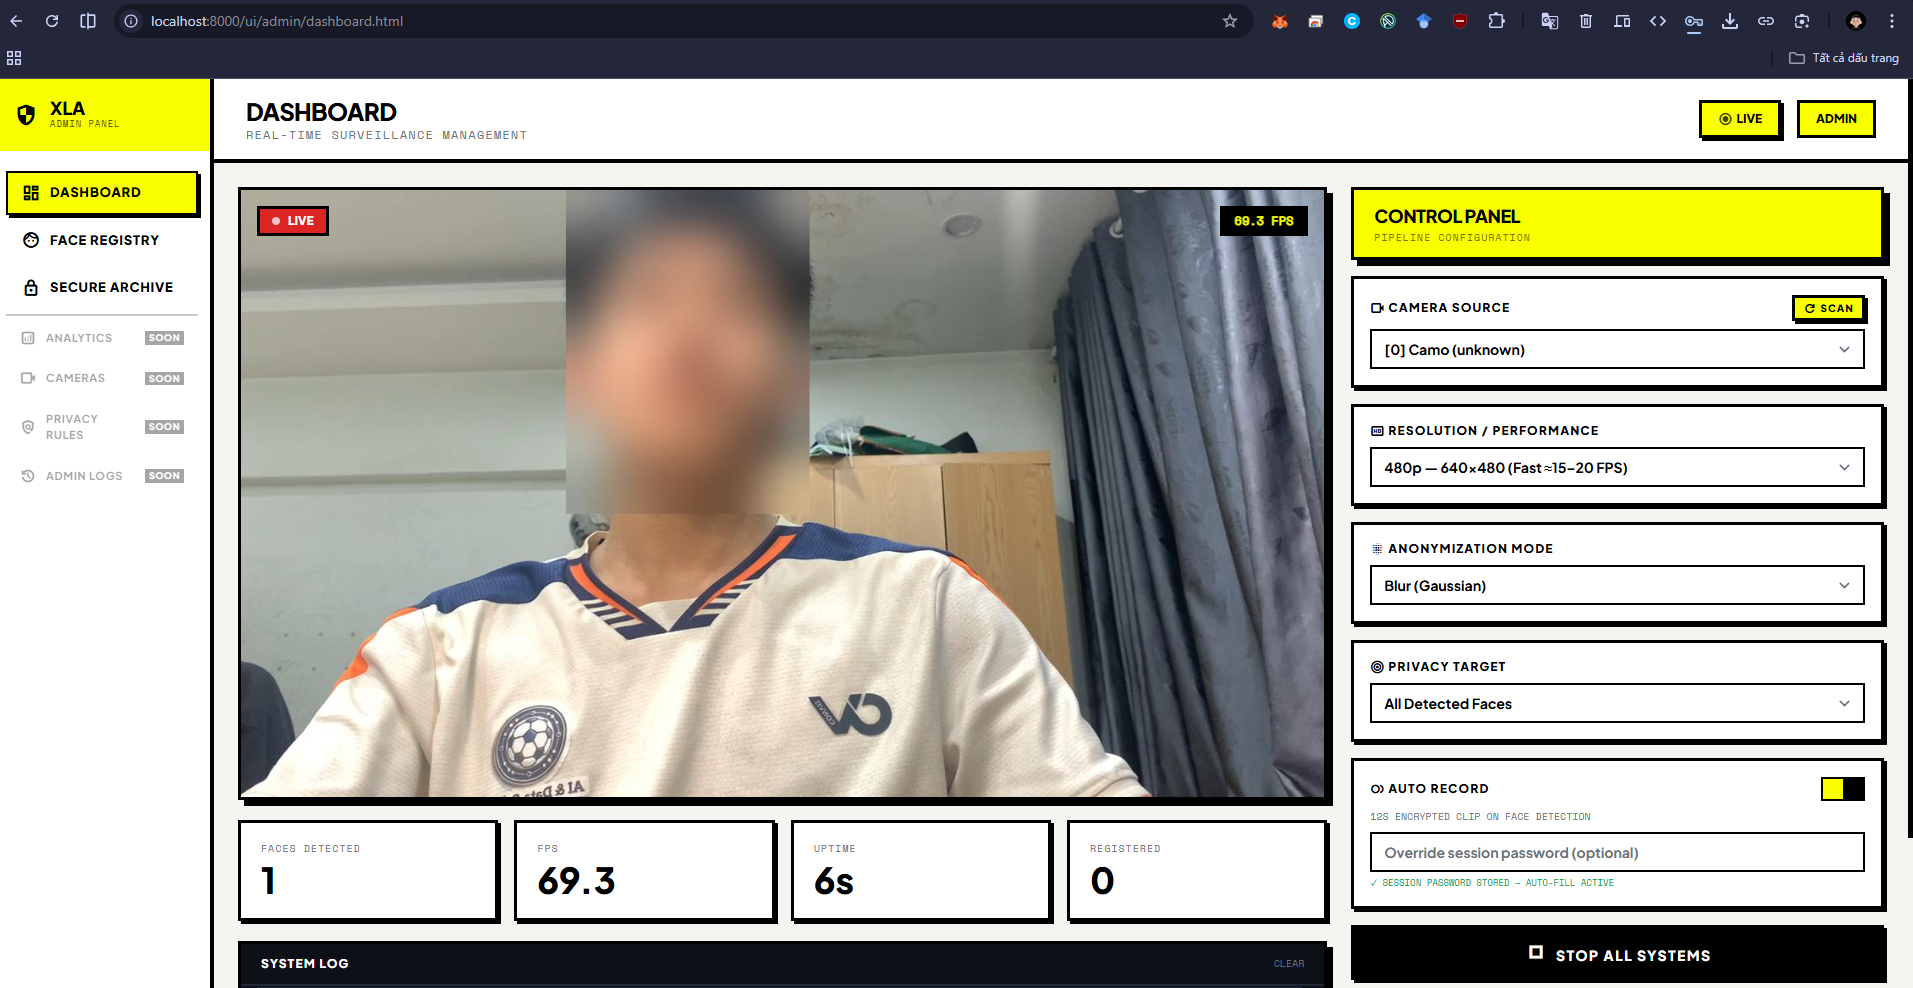
\includegraphics[width=\linewidth]{img/blur.png}\\[2pt]{\small blur}
\end{minipage}\hfill
\begin{minipage}{0.32\textwidth}\centering
  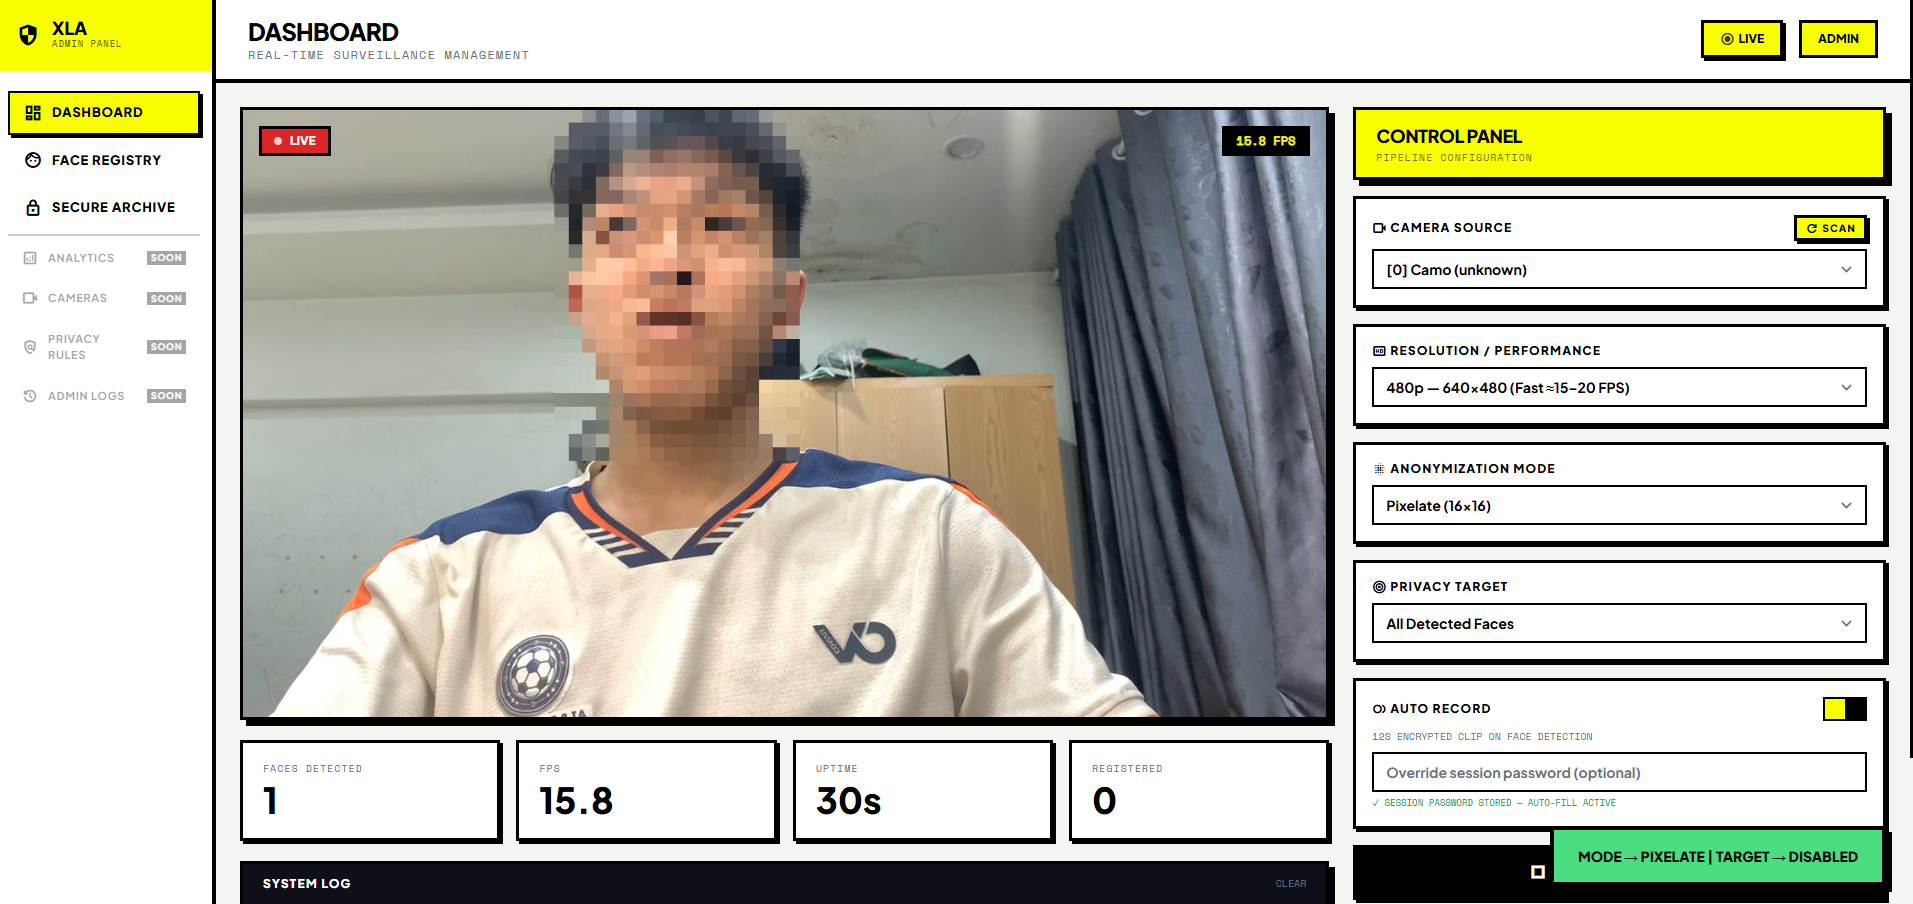
\includegraphics[width=\linewidth]{img/pixelate.png}\\[2pt]{\small pixelate}
\end{minipage}\hfill
\begin{minipage}{0.32\textwidth}\centering
  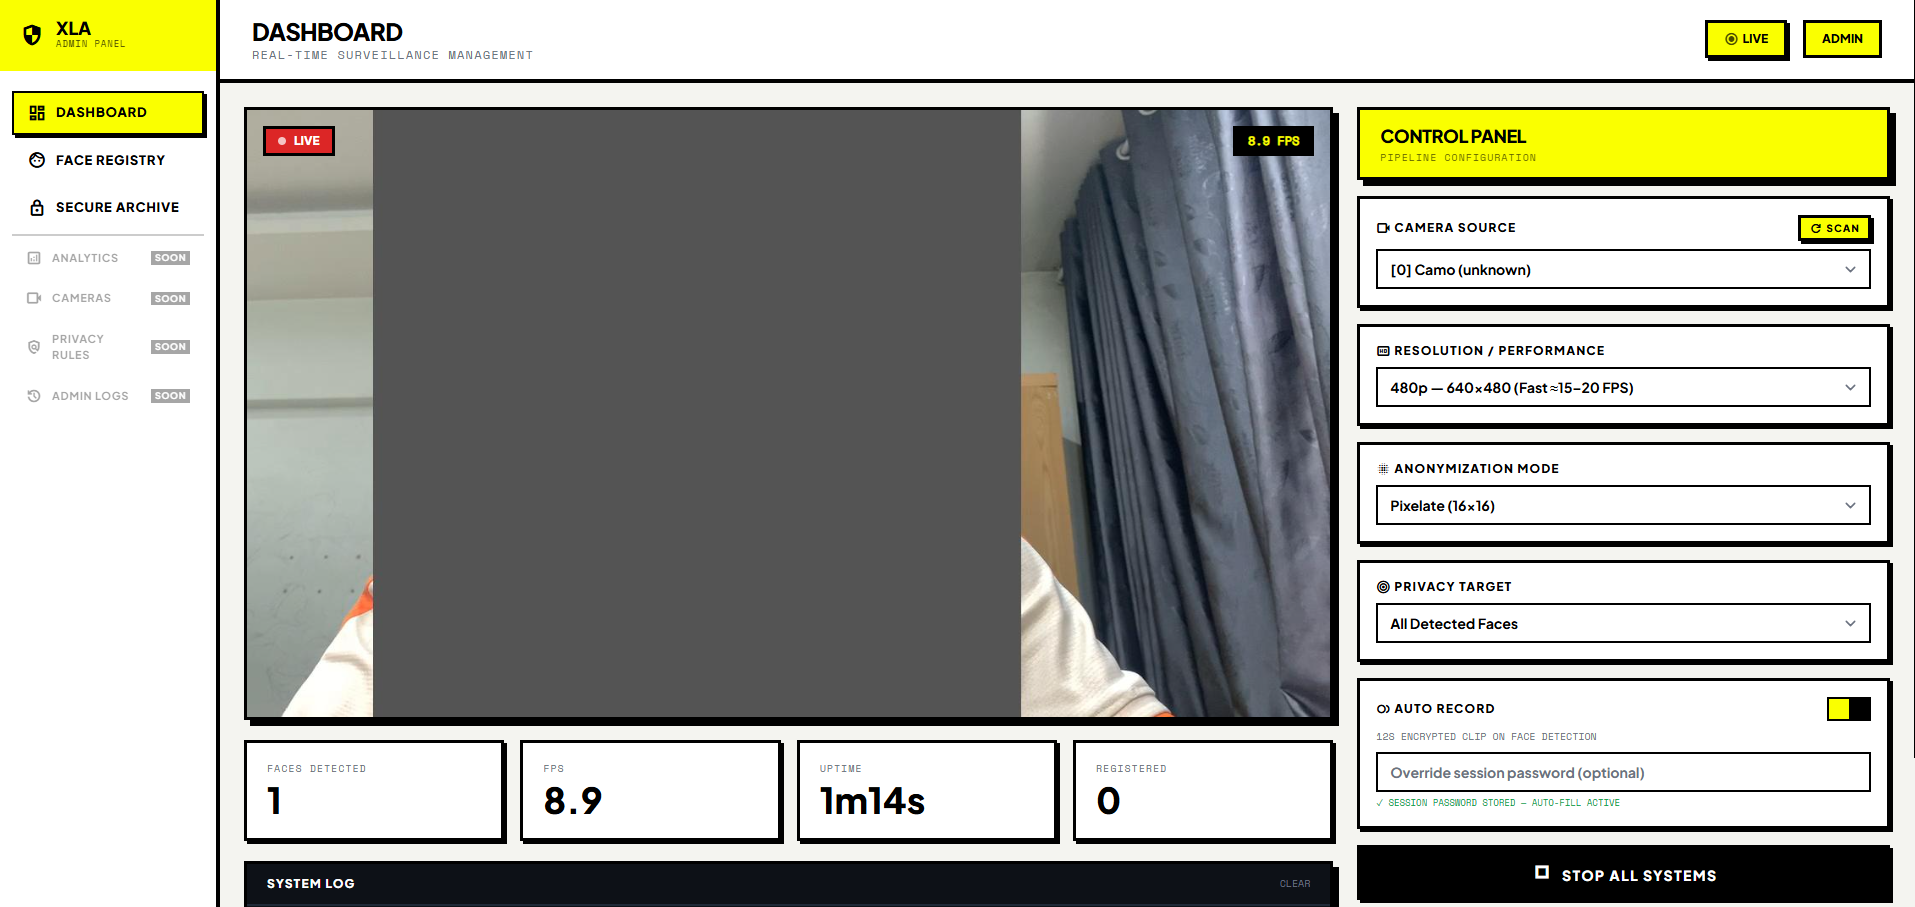
\includegraphics[width=\linewidth]{img/headcloak.png}\\[2pt]{\small headcloak}
\end{minipage}
\\[0.4cm]
\begin{minipage}{0.32\textwidth}\centering
  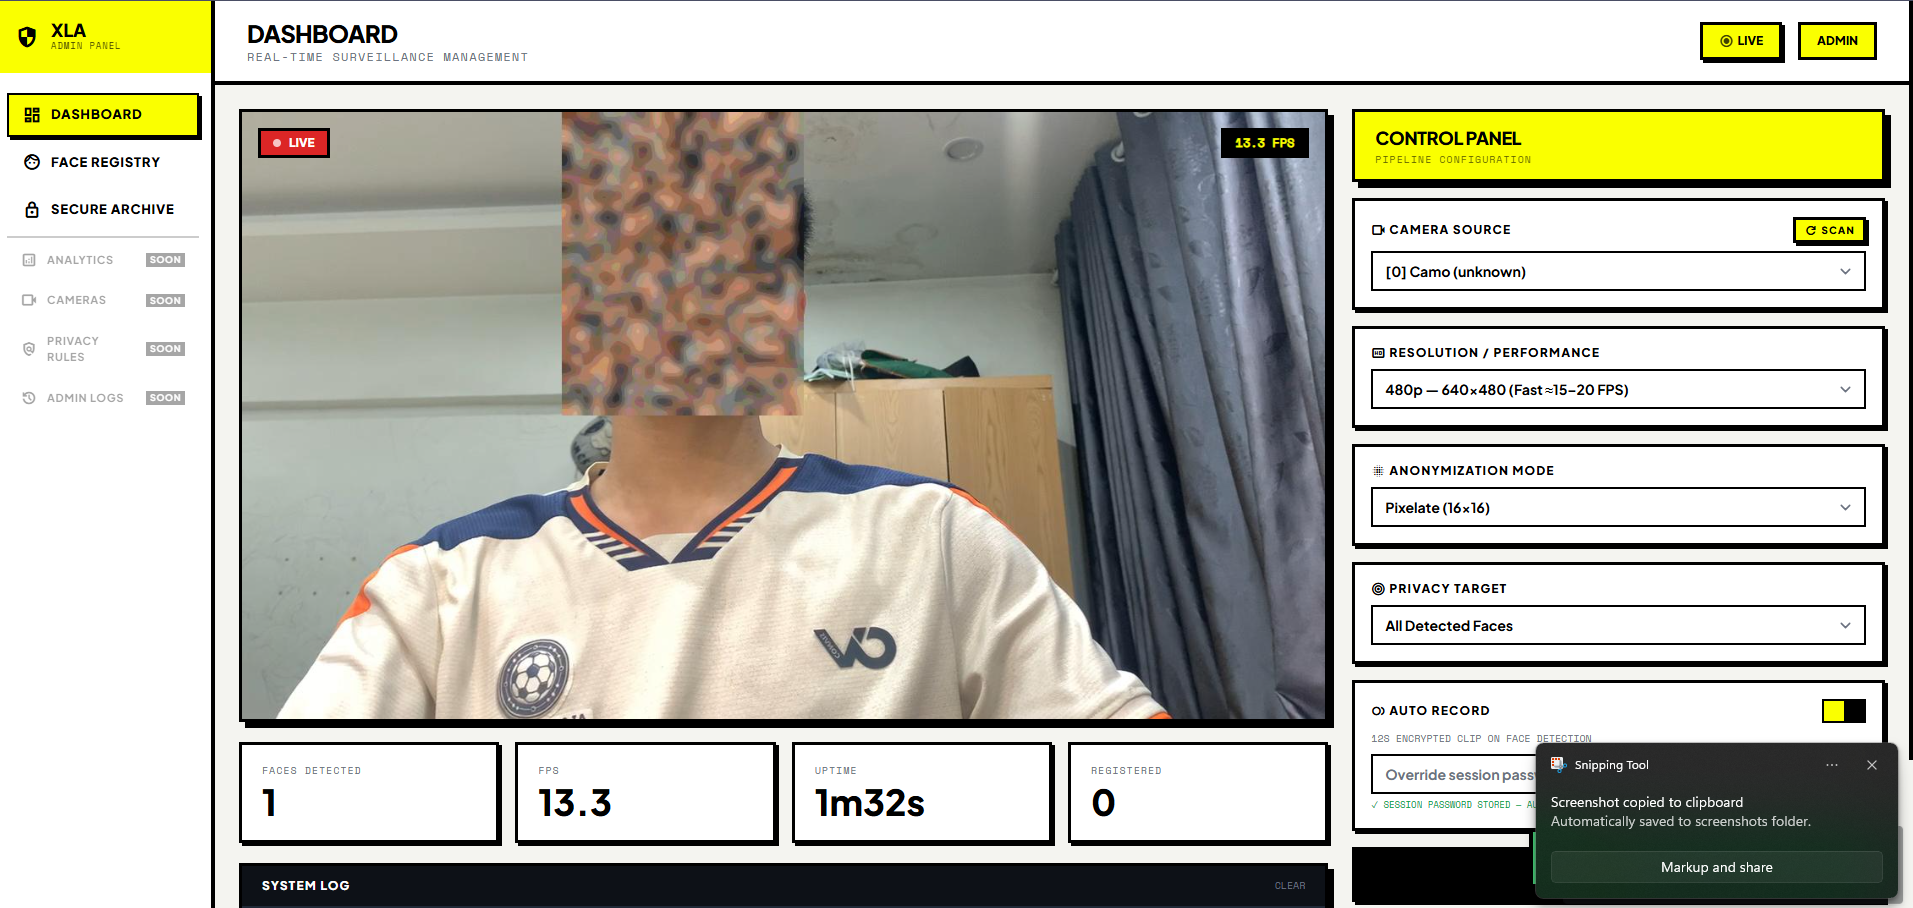
\includegraphics[width=\linewidth]{img/obliterate.png}\\[2pt]{\small obliterate}
\end{minipage}\hfill
\begin{minipage}{0.32\textwidth}\centering
  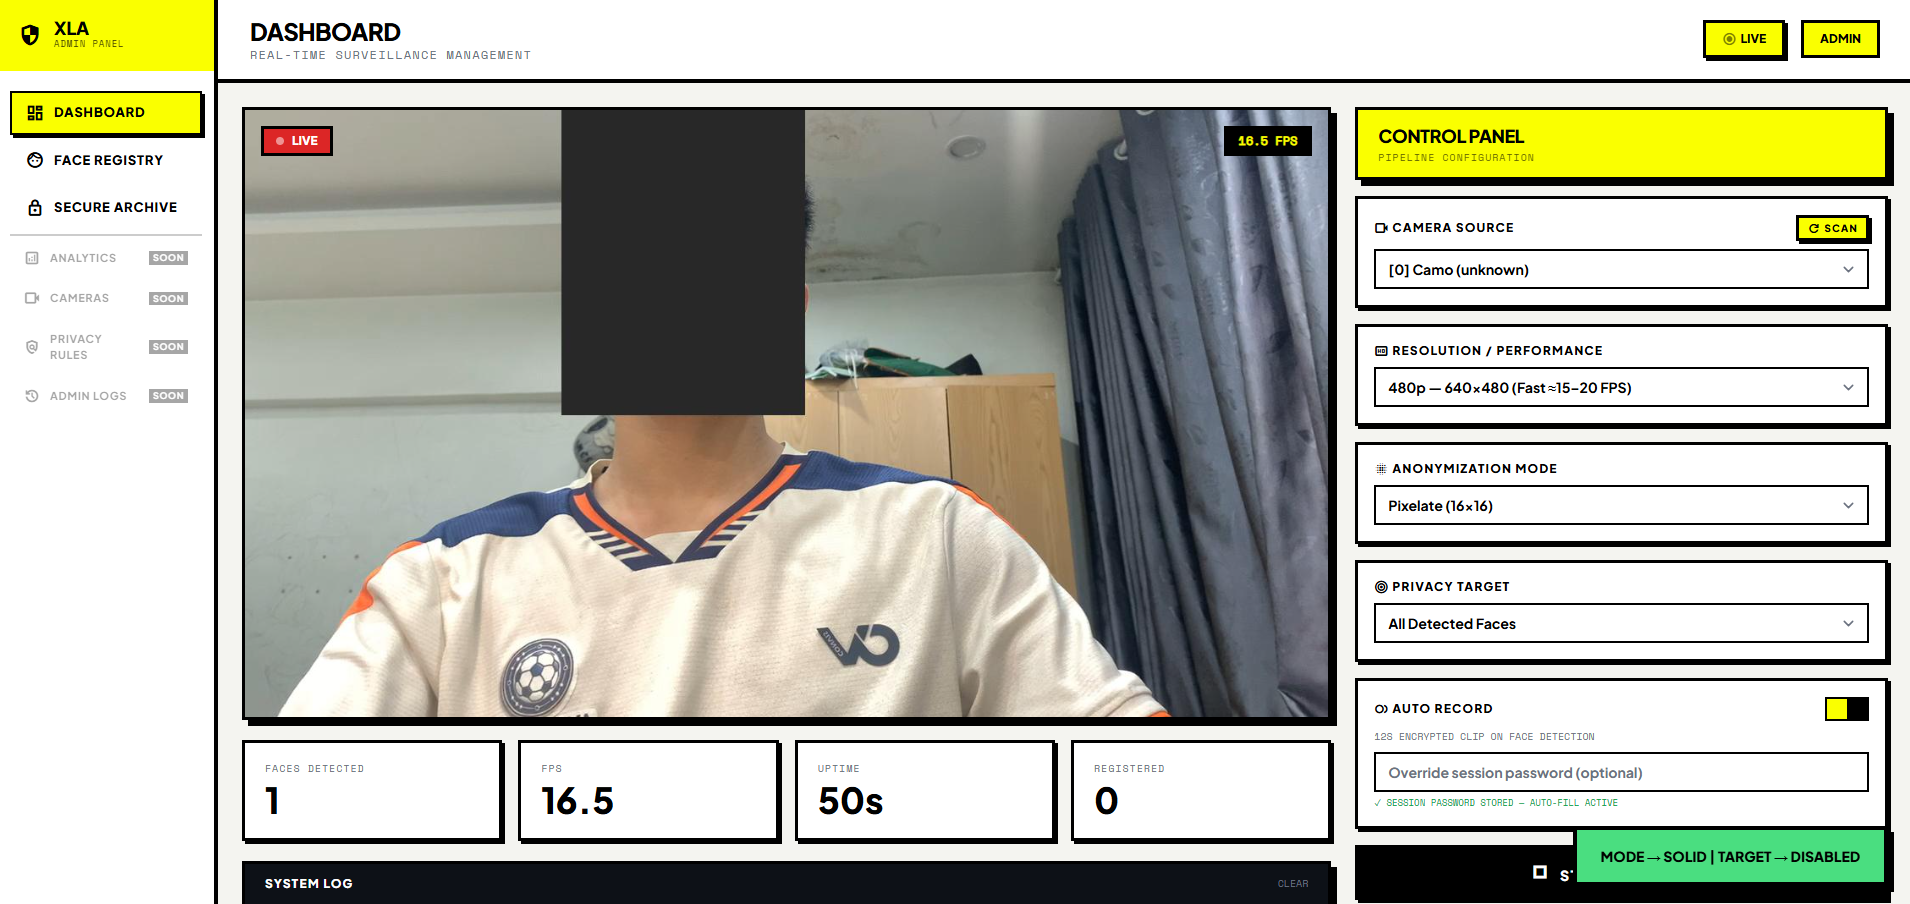
\includegraphics[width=\linewidth]{img/solid.png}\\[2pt]{\small solid}
\end{minipage}\hfill
\begin{minipage}{0.32\textwidth}\centering
  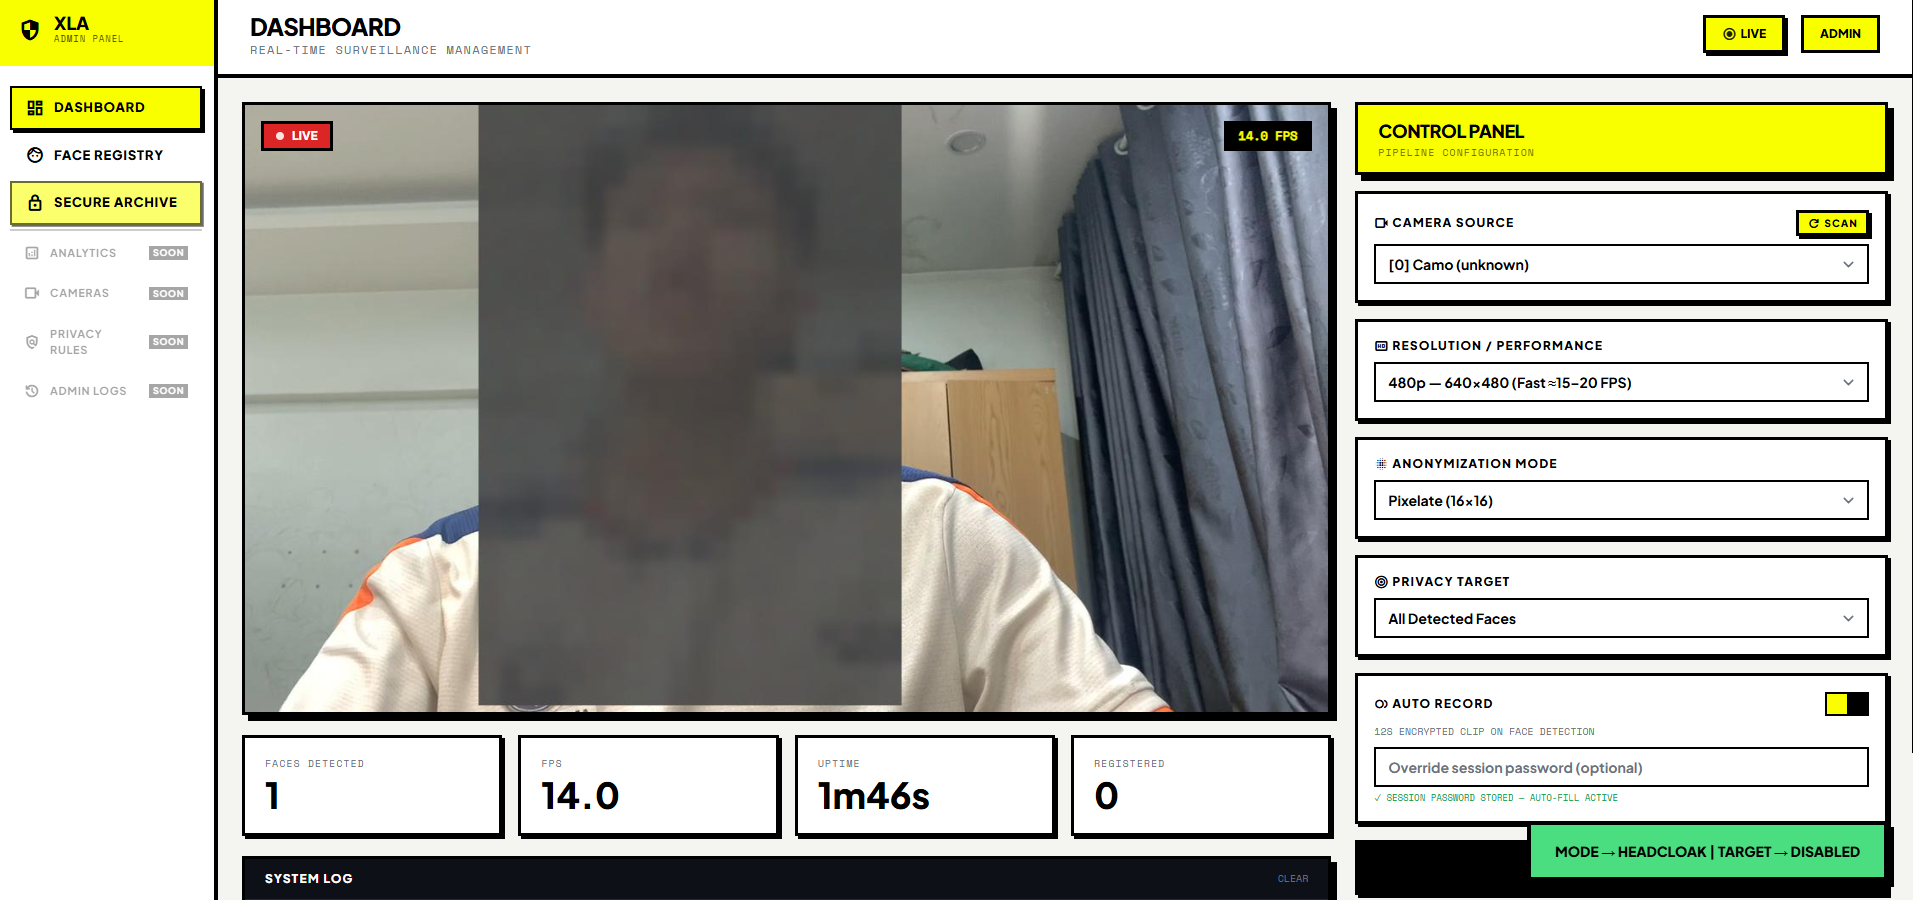
\includegraphics[width=\linewidth]{img/silhouette.png}\\[2pt]{\small silhouette}
\end{minipage}
\caption{So sánh 6 chế độ ẩn danh hoá trên cùng một khung hình thực tế. Từ trái-trên: blur, pixelate, headcloak; dưới: obliterate, solid, silhouette.}
\label{fig:modes_compare}
\end{figure}

\subsubsection{Giao diện web Admin Dashboard}

\begin{figure}[H]
\centering
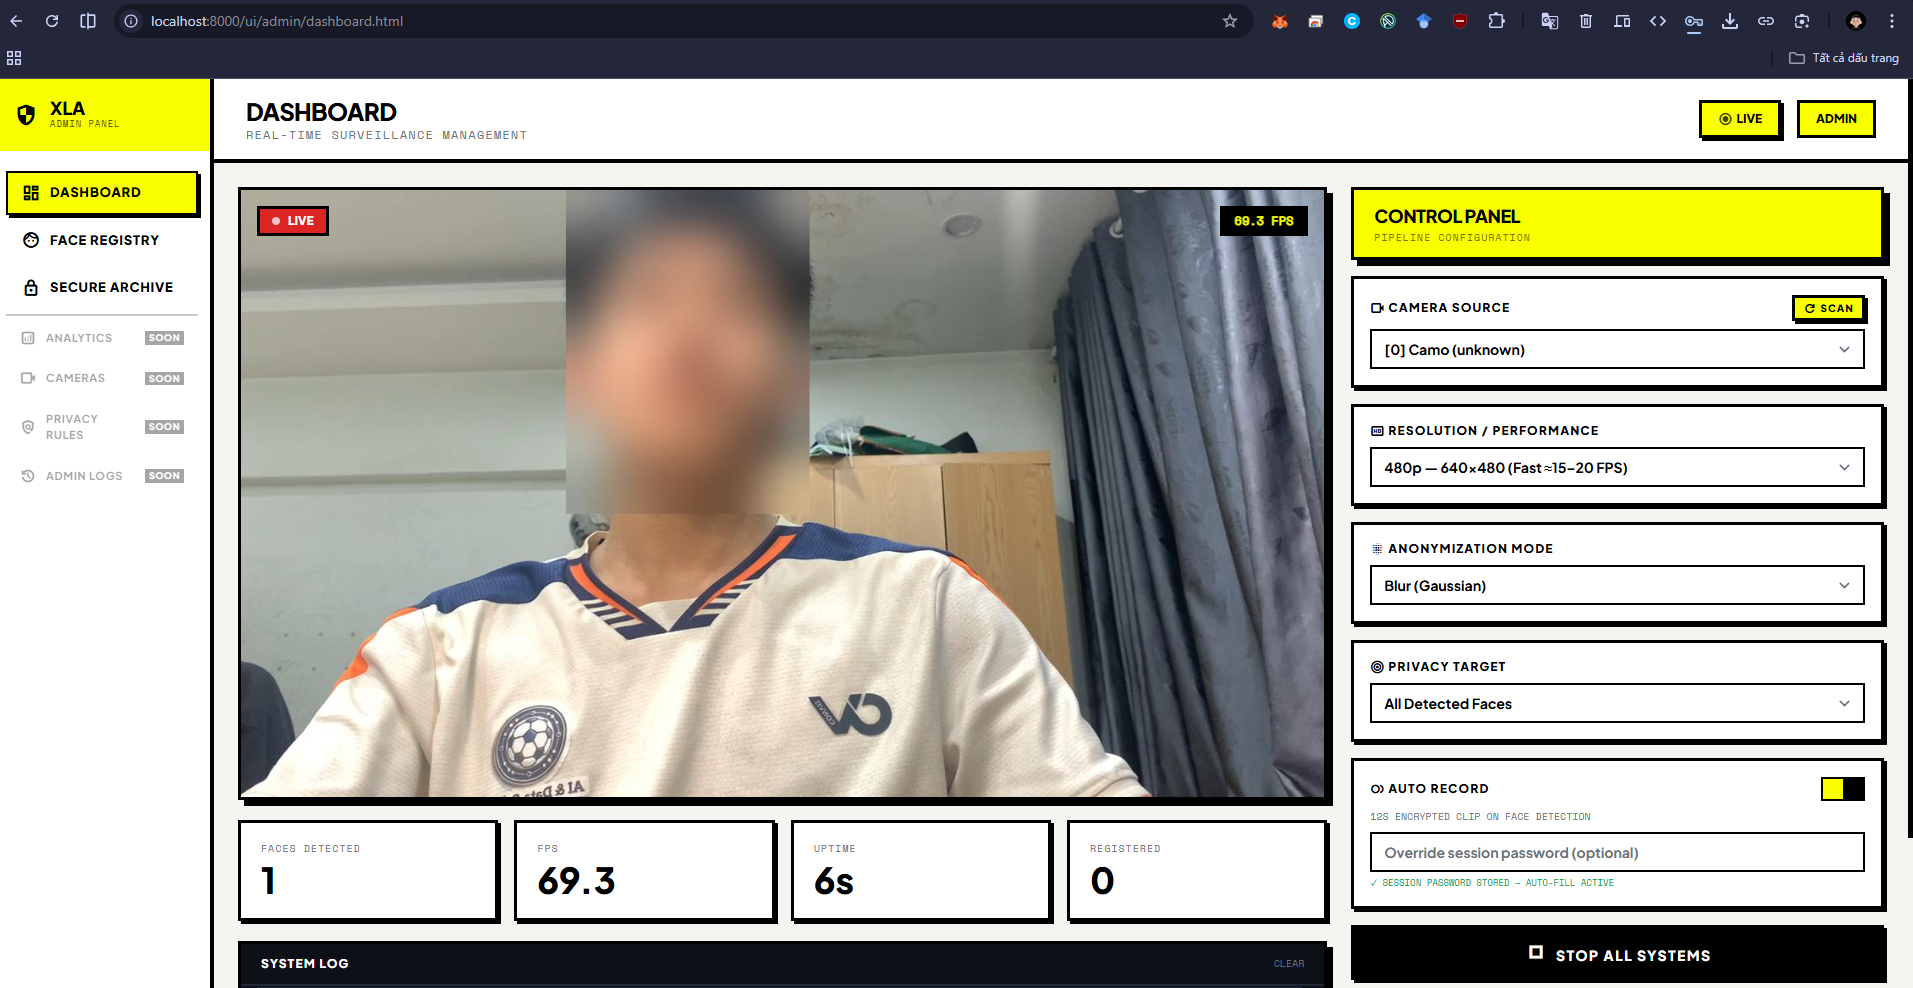
\includegraphics[width=0.95\textwidth]{img/admin_dashboard.png}
\caption{Giao diện Admin Dashboard hiển thị luồng video trực tiếp với chế độ blur đang hoạt động.}
\label{fig:admin_dashboard}
\end{figure}

\subsubsection{Giao diện người dùng --- Live Portal}

\begin{figure}[H]
\centering
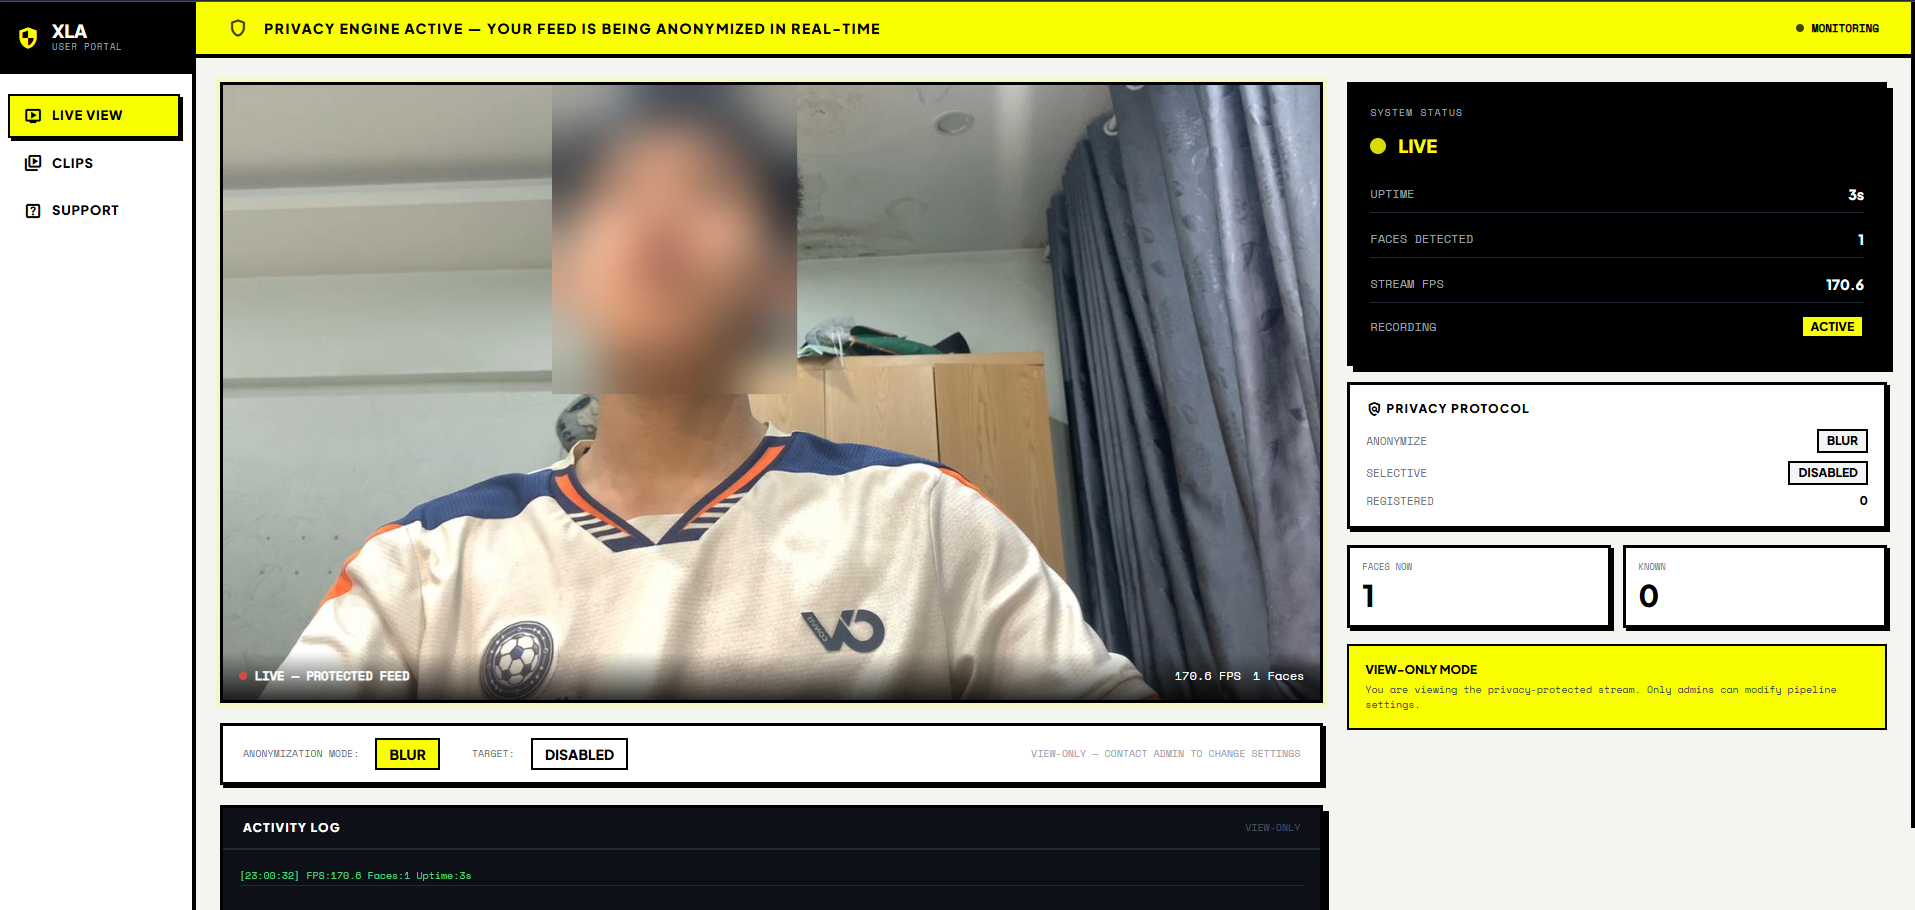
\includegraphics[width=0.95\textwidth]{img/user_portal.png}
\caption{Giao diện User Portal --- Live View. Khuôn mặt đã được ẩn danh hoá, người dùng thường không thể xem bản gốc.}
\label{fig:user_portal}
\end{figure}

\subsubsection{Biểu đồ so sánh FPS theo chế độ}

\begin{figure}[H]
\centering
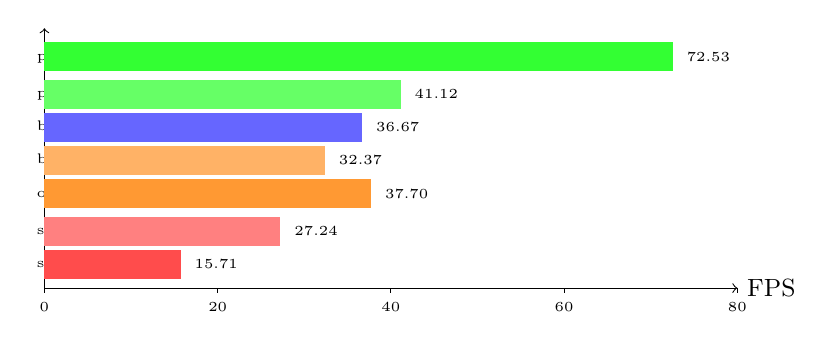
\begin{tikzpicture}
\begin{scope}[xscale=0.11, yscale=0.06]
% Axes
\draw[->] (0,0) -- (80,0) node[right]{\small FPS};
\draw[->] (0,0) -- (0,55);
% Y labels (mode names)
\foreach \name/\y in {
  {silhouette/strong}/5,
  {silhouette/fast}/12,
  {obliterate/str}/20,
  {blur/strict}/27,
  {blur/balanced}/34,
  {pixelate/bal}/41,
  {pixelate/fast}/49
}{
  \node[right, font=\tiny] at (-2, \y) {\name};
}
% Bars
\fill[red!70]      (0,2) rectangle (15.71,8);
\fill[red!50]      (0,9) rectangle (27.24,15);
\fill[orange!80]   (0,17) rectangle (37.70,23);
\fill[orange!60]   (0,24) rectangle (32.37,30);
\fill[blue!60]     (0,31) rectangle (36.67,37);
\fill[green!60]    (0,38) rectangle (41.12,44);
\fill[green!80]    (0,46) rectangle (72.53,52);
% Value labels
\foreach \val/\y in {15.71/5, 27.24/12, 37.70/20, 32.37/27, 36.67/34, 41.12/41, 72.53/49}{
  \node[font=\tiny, right] at (\val+0.5, \y) {\val};
}
% X axis ticks
\foreach \x in {0,20,40,60,80}{
  \draw (\x, 0) -- (\x, -1);
  \node[below, font=\tiny] at (\x, -1) {\x};
}
\end{scope}
\end{tikzpicture}
\caption{So sánh FPS theo chế độ và preset (CPU-only, 100 frame). Xanh lá = hiệu suất cao, đỏ = thấp. Đường 25 FPS là ngưỡng real-time tối thiểu.}
\label{fig:fps_chart}
\end{figure}
